\section{Arrivé sur Bali}

7 avril 2008

\begin{multicols}{2}

Salut tout le monde !!! Bon alors, autant vous le dire tout de suite, vu les photos qui sont dans cet article, vous allez me détester quand vous les aurez vues... enfin disons qu'il y a de fortes chances... Arrivé mercredi, sans aucun souci durant le trajet, Patrick est venu me chercher à l'aéroport pour aller au bateau, joli canot de 13m50, bien équipé pour la navigation, spacieux. Nous sommes allés faire un petit tour à Kuta, coin le plus touristique de Bali, Plage très appréciée des surfers du monde entier. En fait j'ai adoré le passage ombragé qui longe la route et la plage, où une multitude des petits vendeurs proposent location de planche de surf, boissons fraîches et massages, vraiment très tentant.

%\hspace*{-0.65cm}
%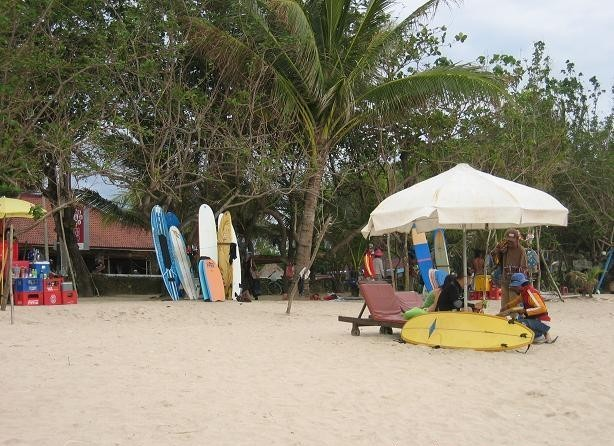
\includegraphics[width=4.8cm]{articles/Arrivee-sur-bali/1207567562ikVd.jpg}
%Plage de Kuta.

Sylvie, une amie de Patrick, est arrivée avec sa fille Tamara le soir, pendant que j'étais dans les bras de Morphée, décalage horaire oblige. Nous somme partis jeudi et revenus samedi matin pour faire un tour dans Bali, en s'arrêtant dans des petits hôtels bien sympathiques (c'est un euphémisme) avec vue sur mer, cocotiers, piscines, eau à 30 degrés quand elle est froide...

%\hspace*{-0.65cm}
%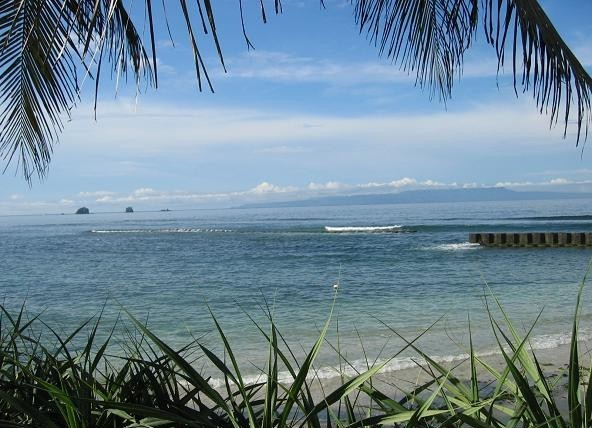
\includegraphics[width=4.8cm]{articles/Arrivee-sur-bali/1207567561DqJk.jpg}
%La mer.

%\hspace*{-0.65cm}
%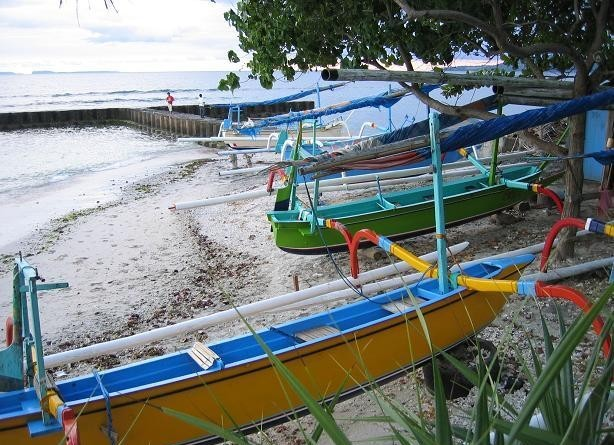
\includegraphics[width=4.8cm]{articles/Arrivee-sur-bali/1207567564x5vI.jpg}
%Bateau de pêche traditionnels.

%\hspace*{-0.65cm}
%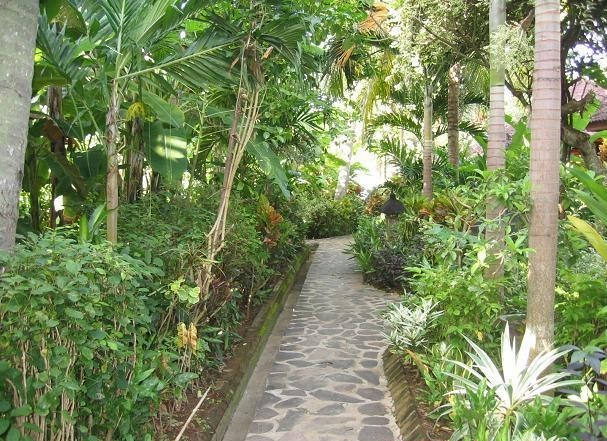
\includegraphics[width=4.8cm]{articles/Arrivee-sur-bali/120756756426sq.jpg}
%L'allée d'un hôtel.

%\hspace*{-0.65cm}
%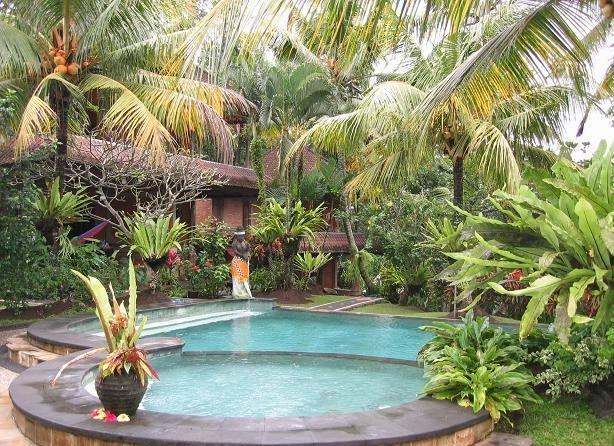
\includegraphics[width=4.8cm]{articles/Arrivee-sur-bali/1207567563njCA.jpg}
%Ze piscine.

La capitale de l'île est Denpasar, ville qui grouille de partout, sans gros interêt à ce que l'on m'a dit, j'irais voir quand même... L'aéroport est à Kuta, juste au Sud de Denpasar, ville beaucoup plus jolie... et touristique. En ce qui me concerne, le bateau est à la Marina de Benoa, juste à l'Est de Kuta. Je connaissais deja un peu l'artisanat de Bali, les balinais font de magnifiques objets de déco, des tissus, des sculptures, on en voit partout. Ici une photo prise au bord de la route dans un petit village.

%\hspace*{-0.65cm}
%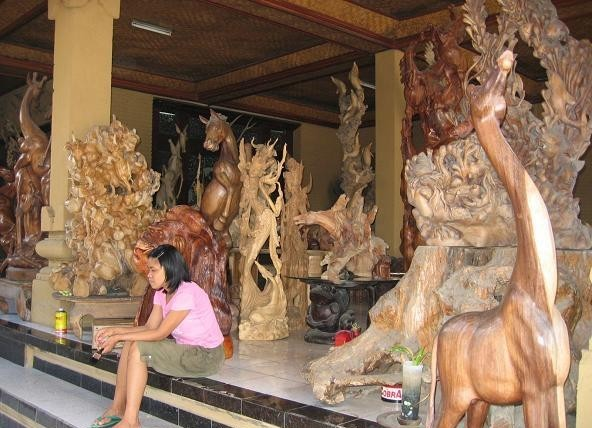
\includegraphics[width=4.8cm]{articles/Arrivee-sur-bali/1207567562ISpn.jpg}
%Sculptures en bois.

Dans les jours qui suivent je vais louer un scooter pour faire un tour complet de l'île, essayer d'aller voir un pote de Patrick, Indonésien, plus au Nord dans l'île, monter sur le plus gros volcan, me perdre dans les rizières, enfin pas trop de plans a l'avance, il est très facile de se loger ici, les gens sont aussi sympa qu'en Inde, et bizarrement l'immense majorité des personnes que l'on voit ont entre 20 et 25 ans.

A bientôt.

\end{multicols}

\bigskip
\textbf{\textsc{Commentaires}}

\medskip
Cécile a écrit le 7 avril 2008 :
\begin{displayquote}
Hum\dots que dire\dots c'était vraiment mieux d'être du côté qui prend la photo :) Pas de doutes ça fait rêver, mais je te déteste même pas, va falloir nous en montrer encore et toujours plus!
Contente que tout se soit bien passé et que tu t'entendes bien avec Patrick. Enjoy!
Gros bisous.
\end{displayquote}

\medskip
Titou a écrit le 8 avril 2008 :
\begin{displayquote}
Hey ti Dud !
Ralalala elles déchirent tes photos ! Comme Cécile je ne te déteste pas mais j'aimerai bien être avec toi là-bàs plutôt qu'assis sur les genoux de Norbert :D
Profites à fond et je suis bien content que tu sois au paradis ! éclates toi et fais gaffe quand même !
A plus mon pote !
\end{displayquote}

\medskip
Gégé a écrit le 8 avril 2008 :
\begin{displayquote}
Ben moi je te déteste, pas comme les deux autres\dots
À Belfort plage, en ce moment on se gèle les roubignoles, il fait pas loin de 0, le vent nous glace les os et il neige ou il pleut (ça dépend si on est dans le plus froid que 0 ou plus chaud). Bref : bêêêêê.
Vivement un chtiot bout de printemps.
++, have fun.
\end{displayquote}

\medskip
Peggy a écrit le 8 avril 2008 :
\begin{displayquote}
A Mornant les bains le temps n'est pas au beau fixe et ton message / photo illumine la journée.
Quelle chance!
Je pense que tu dois vraiment apprécier ce confort après avoir vécu une expérience totalement différente il y a peu
ENJOY IT.
\end{displayquote}

\medskip
Jean Yves a écrit le 9 avril 2008 :
\begin{displayquote}
Il y 2 jours il y avait ici à St Maurice 2 cm de glace qui empêchaient d'ouvrir un volet le matin\dots Alors avoir des images qui vous narguent ainsi, en provenance directe du Paradis, ça devrait être interdit\dots
\end{displayquote}

\medskip
Etienne a écrit le 10 avril 2008 :
\begin{displayquote}
Pour tout vous dire en arrivant ici je m'attendais à voir de très beaux paysages, mais je suis quand même bluffé.
Aujourd'hui je suis en scooter dans les rizières, à l'Ouest de l'île et vous verrez dans mon prochain post que ça vaut le détour, là aussi.
Il faut quand même que je fasse une petite précision : les photos d'hôtels que vous voyez ici sont des hôtels de bonne catégorie, peu chers car hors saison, (130.000 Rupiah pour deux, 1 euro = 14.000 Rupiah) mais ce n'est pas dans ce genre d'hôtel que je vais quand je suis seul comme ces jours ci.
Merci pour vos messages de soutient dans ces durs moments que je traverse\dots et à bientot.
\end{displayquote}

\medskip
Arnaud a écrit le 13 avril 2008 :
\begin{displayquote}
De magnifiques paysages que tu traverses là mon très cher Dud ! Ca laisse rêveur en tout cas !
Amène nous un peu de soleil\dots juste un peu (on demande pas beaucoup) :D
Bon voyage @ toi
++
\end{displayquote}

\medskip
Etienne a écrit le 14 avril 2008 :
\begin{displayquote}
Ok Arnaud\dots mais tu m'envoies des m\&m's (ah bah oui\dots monsieur est en stage chez mars).
\end{displayquote}

\medskip
Lara a écrit le 29 avril 2008 :
\begin{displayquote}
Coucou p'tit cousin eh ben t'es dans un pays magnifique est très ressourçant profites de cette chance j'te dis à très vite j'espère, bisoussss. Vis ton voyage à fond.
\end{displayquote}

\medskip
Etienne a écrit le 30 avril 2008 :
\begin{displayquote}
Salut Lara, ça me fait plaisir de te voir ici !
\end{displayquote}

\vfill

